Tässä luvussa esitetään perusteet ja tarvittavat tiedot hyväksymistestauksesta, johon testauksen tasoista tässä diplomityössä keskitytään.
Ensin esitetään hyväksymistestauksen tarkoitus, jonka jälkeen keskitytään hyväksymistestausvetoiseen kehitykseen ja sen esittelemiseen ohjelmistotuotannollisena menetelmänä.
Hyväksymistestausvetoisen kehityksen jälkeen käydään läpi web-sovelluksien yhteydessä huomioitavia erityispiirteitä hyväksymistestauksen toteuttamisen näkökulmasta.
Web-sovelluksien erityispiirteiden jälkeen esitetään tämän diplomityön yhteydessä kehitetyn hyväksymistestausjärjestelmän rakentamiseen käytettyjä, mutta kuitenkin myös hyvin yleisiä hyväksymistestauksen työkaluja.
Testausjärjestelmän rakenteen lisäksi käydään omassa kappaleessaan myös läpi testitapauksien rakentaminen painottuen testausjärjestelmässä käytettyihin työkaluihin.
Lopuksi esitetään yleisestikin ottaen testitapauksiin tärkeästi liittyvä priorisointiongelma, pyritään esittämään miksi sen ratkaiseminen on tärkeää ja esitetään erilaisia menetelmiä sen ratkaisemiseen.

\section{Hyväksymistestauksen tarkoitus} \label{ch:08_hyvaksymistestauksen_tarkoitus}

  Hyväksymistestaus on testauksen tasoista tärkeimpiä, sillä sen ollessa kattava, voidaan verifioida ohjelman toiminta korkealla tasolla saaden samalla varmuus siitä, että hyväksymistestausta alemmilla tasoilla testattavat asiat toimivat riittävän oikein.
  Hyväksymistestauksen tarkoituksena on varmistaa toteutettavan ohjelmiston vaatimusten toimivuus erityisesti käytännön tilanteissa siten, että voidaan varmistaa vastaako ohjelmisto loppukäyttäjän tarpeita.
  Hyväksymistestaus antaa vastauksen siihen, toimiiko toteutettu järjestelmä loppukäyttäjän tarpeiden mukaisesti ja loppukäyttäjän näkökulmasta oikein.
  Hyväksymistestauksen sanotaan olevan muodollista testaamista, jossa käyttäjän tarpeet, vaatimukset ja liiketoimintaprosessit otetaan huomioon selvittäessä täyttääkö järjestelmä hyväksymisen kriteerit ja sallii auktorisoidun tahon päättää hyväksytäänkö järjestelmä julkaistavaksi \parencite{istqb_acceptance_testing_1}.
  Ohjelmistotestauksen tekniikoiden näkökulmasta hyväksymistestaus on mustalaatikkotestausta, eli testauskohdetta testataan tietämättä sen teknisestä toteutuksesta.
  Hyväksymistestauksen painoarvo on asiakasperusteisessa vaatimusmäärittelyssä ja loppukäyttäjän tarpeiden kartoittamisessa.
  Testiautomaation osalta hyväksymistestausta varten voidaan rakentaa testitapaukset, joiden avulla voidaan keskittyä varmistamaan loppukäyttäjille tarpeellisten toimintojen toteutuminen testitapauksien suorittamisen jälkeen.
  Hyväksymistestauksen osalta testitapauksia voidaan toteuttaa niin sanotulla päästä päähän -periaatteella, jossa testattavaa järjestelmää testataan siten kuin loppukäyttäjä sitä käyttäisi.
  Hyväksymistestauksessa ei anneta painoarvoa esimerkiksi kosmeettisille tai kirjoitusvirheille, vaan pyritään selvittämään loppukäyttäjille oleellisten ja tarpeellisten toimintojen toteutuminen.

  Hyväksymistestaus on aiemmin esitetyistä testauksen tasoista \ref{ch:07_testauksen_tasot} viimeinen ja sen suorittamisen jälkeen saadaan tieto, onko järjestelmä toteutuksen osalta sellaisenaan valmis julkaistavaksi.
  Perinteisesti hyväksymistestauksen lähtökohtia ovat selvät hyväksymisvaatimukset sekä julkaisukelpoinen toteutus joka voi sisältää vain kosmeettisia tai kirjoitusvirheitä.
  Hyväksymisvaatimukset voivat olla esimerkiksi liiketoiminnallisia käyttötapauksia, prosessivirtauskaavioita sekä vaikkapa ohjelmiston vaatimusmäärittely.
  Testiautomaatiota varten käytettävästä testialustasta riippuen hyväksymistestauksen käyttötapaukset voidaan muodostaa joko osittain tai suoraan testitapauksiksi.
  Hyväksymistestaukseen usein pyydetään osallisiksi ohjelmistokehittäjien lisäksi myös muita sidosryhmiä ja toisinaan jopa loppukäyttäjiä.
  Keskeistä on, että loppukäyttäjiltä hankitaan tieto tarvittavista ja toteutettavista ominaisuuksista, kun taas muut sidosryhmät kuten esimerkiksi johtoryhmä voivat tehdä liiketoiminnallisia päätöksiä hyväksymistestauksen onnistumisen osalta ja esimerkiksi peruuttaa julkaisun.
  Hyväksymistestaus siis antaa mahdollisuuden korjata usein liiketoiminnallisestakin näkökulmasta merkittävät toiminnalliset virheet ennen järjestelmän julkaisua loppukäyttäjille.

  Kehittäjien käsitys järjestelmän toiminnallisuudesta ja sen vaatimuksista voi kuitenkin olla usein hyvinkin erilainen kuin loppukäyttäjien.
  Hyväksymistestauksen avulla voidaan lievittää tätä ongelmaa, ja saada ohjelmistokehittäjät loppukäyttäjien kanssa vaatimusmäärittelyn suhteen samalle aaltopituudelle.
  Testiautomaation avulla toteutettavalla toistuvalla hyväksymistestauksella varmistetaan, että järjestelmä toteuttaa loppukäyttäjän tarpeet vielä järjestelmään tehtyjen muutoksien jälkeenkin.
  Hyväksymistestauksen testitapaukset tarkoituksenmukaisesti heijastavat suoraan loppukäyttäjien tarpeita, jonka avulla ohjelmistokehittäjät ja muut sidosryhmät voivat tehokkaasti varmistaa järjestelmän valmiuden ja sen hetkisen tilan.
  Hyväksymistestauksella siis saadaan katsaus ohjelmiston valmiudesta sen vaatimuksiin ja loppukäyttäjien toiminnallisiin tarpeisiin nähden.

\section{Hyväksymistestausvetoinen kehitys} \label{ch:08_hyvaksymistestausvetoinen_kehitys}

  Hyväksymistestausvetoisen kehityksen tarkoituksena, kuten testausvetoisessakin kehityksessä on toteuttaa ohjelmistotuotannollinen prosessi laatien toistettavasti suoritettavat testitapaukset ennen ohjelmiston varsinaista toteutusta.
  Hyväksymistestausvetoisessa kehityksessä tämä tarkoittaa käytännössä sitä, että ennen toteutusta luodaan tarvittavat ohjelmiston asiakasvaatimuksia palvelevat hyväksymistestit, jotka ohjelmiston on tarkoitus läpäistä sen julkaisemisen hyväksymiseksi.
  Hyväksymistestausvetoisen kehityksen sanotaan olevan yhteistyöhön perustuva lähestymistapa kehitykseen, jossa tiimi ja asiakkaat käyttävät asiakkaiden oman ympäristön kieltä ymmärtääkseen heidän vaatimukset, jotka muodostavat pohjan komponentin tai järjestelmän testaamiseen \parencite{istqb_acceptance_testing_2}.
  Tarvittavat ohjelmiston hyväksymistestit suoritetaan iteratiivisesti ohjelmistokehitysprosessin aikana ja se tarkoittaa käytännössä jatkuvan integraation ottamista käyttöön ohjelmistokehityksessä.
  Hyväksymistestausvetoinen kehitys on erittäin hyödyllinen ohjelmistokehityksessä käytetty menetelmä, sillä kehitysvaiheessa on aina tarkasti tiedossa, vastaako ohjelmiston sen hetkinen tila asiakasvaatimuksia ja kuinka hyvin se niiden täyttämisessä onnistuu.

  \begin{figure}[H]
    \centering
    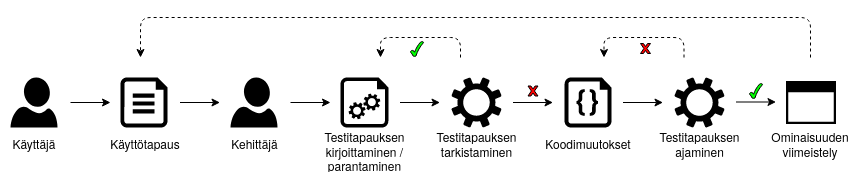
\includegraphics[width=0.8\textwidth]{assets/hyvaksymistestausvetoinen-kehitys.png}
    \caption{Hyväksymistestausvetoisen kehityksen vaiheet}
    \label{fig:hyvaksymistestausvetoinen-kehitys}
  \end{figure}

  Hyväksymistestausvetoinen kehitys on sen yläkäsitteen, testausvetoisen kehityksen, kanssa perusperiaatteeltaan samanlainen, mutta ennen ohjelmistokehityksen aloitusta asiakasvaatimukset kartoitetaan ja ohjelmiston hyväksyttävyys määritellään.
  Hyväksymistestitapaukset kirjoitetaan testausvetoisen kehityksen mukaisesti ennen toteutusta ja ohjelmistokehitys itsessään noudattaa iteratiivisesti testausvetoista kehitystä, vaikkakin hyväksymistestaus on perinteisesti vaatinut lähes valmista järjestelmää \parencite{traditional_acceptance_testing}.
  Asiakasvaatimukset määritetään usein käyttötapauksien muodossa ja hieman testialustasta riippuen ne voidaan kirjottaa suoraan testitapauksien muotoon.
  Hyväksymistestausvetoisessa kehityksessä ohjelmistokehitystä ohjaavat asiakasvaatimukset ja loppukäyttäjien tarpeiden toteutuminen, jotka ovat hyvin usein toiminallisia vaatimuksia.
  Hyväksymistestausvetoisessa kehityksessä mitataan jatkuvasti käyttötapauksien muodossa validoitavien haluttujen ominaisuuksien toteutumista.
  Perusperiaate on kirjoittaa asiakasvaatimus tai käyttötapaus testitapauksen muotoon, toteuttaa testitapaus, ajaa testitapaus läpäisemättömänä, toteuttaa ominaisuus, ajaa testitapaus läpäisevänä, refaktoroida toteutus ja siirtyä takaisin seuraavaan käyttötapaukseen.
  Käyttötapaus koostuu rakenteellisesti usein tilanteesta, motivaatiosta ja halutusta lopputuloksesta.
  Esimerkki käyttötapauksesta voi olla: \emph{käyttäjänä, haluan sisäänkirjautumisen jälkeen voida avata premium ominaisuudet tekemällä sovelluksensisäisen oston}.

  Hyväksymistestausvetoisessa kehityksessä hyväksymistestit ovat hyödyllistä pilkkoa pieniin hallittaviin kokonaisuuksiin, jolloin voidaan iteratiivisesti toteuttaa valmiiksi tietyn testitapauksen mukainen ominaisuus, joka vastaa jotakin käyttötapausta tai loppukäyttäjän tarvetta.
  Hyväksymistestauksessa testitapaus voi olla esimerkiksi käyttäjän tietojen muuttumisen varmistaminen, kuten tason läpäiseminen pelisovelluksessa, joka muuttaa käyttäjän edistystä.
  Menetelmänä hyväksymistestausvetoisen kehityksen tarkoituksena on onnistua vastaamaan loppukäyttäjän tarpeisiin tehokkaasti ja hyvin ottamalla tarpeet huomioon jo ennen toteutuksen aloittamista.
  Menetelmän avulla myös luodaan ymmärrystä ohjelmistotuotteen valmiuden määritelmästä, kun eri sidosryhmän voidaan saada sen suhteen samalle aaltopituudelle.
  Hyväksymistestausvetoinen kehitys on lisäksi erittäin hyödyllistä, sillä jatkuva testaaminen antaa mahdollisuuden haluttujen ominaisuuksien toteutumisen validoimiselle menetelmän jokaisen iteraation koontiversiossa.

\section{Web-sovelluksien erityispiirteet} \label{ch:08_websovelluksien_erityispiirteet}

  Web-sovelluksilla on omia erityispiirteitä, jotka vaikuttavat testitapauksien laatimiseen.
  Nykypäivänä web-sovellukset ovat kasvaneet kompleksisuudessa ja front-end puolen toteutuksia tarkasteltaessa web-sovellukset usein muistuttavat jo perinteisiä dynaamisia työpöytäsovelluksia.
  Web-sovelluksia päivitetään usein tiheään tahtiin, jolloin niille on suuri tarve luoda testiautomaatiota, jota hyödyntäen voidaan varmistaa, että ne toimivat oikein muutoksien jälkeenkin.

  Hyväksymistestauksen priorisoimisen osalta tärkeä web-sovelluksien erityispiirre liittyy käyttöliittymiin ja DOM-dokumenttiobjektimalliin.
  Dokumenttiobjektimallin avulla verkkoselaimet esittävät käyttöliittymän ja siinä näkyvän sisällön.
  Tämän lisäksi dokumenttiobjektimalli mahdollistaa käyttöliittymässä olevien elementtien valitsemisen, jota hyödynnetään vahvasti testitapauksien kirjoittamisessa.

  Navigointi ja navigointiketjut ovat myös yksi web-sovelluksien erityispiirre.
  Historiallisesti verkkosivuilla navigointi tapahtuu niin sanottujen hyperlinkkien avulla, verkkosivujen itse ollessa hypertekstiä.
  Tämä historiallinen lähestymistapa on edelleen käytössä ja web-sovelluksissa on lähes poikkeuksetta useita hyperlinkkejä joiden avulla navigoiminen luo navigointiketjuja, joissa edelliseen sivuun tiedetään palata.
  Hyperlinkkien avulla tapahtuva navigointi ja navigointiketjut ovat sellainen erityispiirre, joka on hyvä tiedostaa myös hyväksymistestauksen testitapauksia rakentaessa.

  Web-sovelluksien syötteet ja niiden yhteyteen liittyvä tietoturva ovat sellainen erityispiirre joka vaatii suurta huomiota.
  Web-sovelluksien syötteisiin on perinteisesti liittynyt paljon haavoittuvuuksia, kuten esimerkiksi XSS-hyökkäykset ja SQL-injektiot.
  Web-sovelluksien hyväksymistestauksen testitapauksiin on hyvä sisällyttää syötteisiin liittyvää testaamista, joissa tietoturva pidetään mielessä.

  Erilaisia web-sovelluksen loppukäyttäjien asiakasympäristöjä on erittäin paljon, joka kannustaa moniselaimellisen testauksen rakentamiseen.
  Näissä ympäristöissä on omat verkkoselaimensa, näyttöresoluutiot ja selainasetukset, jotka saavat saman web-sovelluksen toimimaan eri tavoilla eri ympäristöissä ja luovat siten usein jopa päänvaivaa ohjelmistokehittäjille.
  Etenkin web-käyttöliittymiin keskittyessä testitapauksiin on hyvä sisällyttää erilaisia näyttöresoluutioita, kuvankaappauksien ottamista ja selainasetuksista esimerkiksi JavaScript-ominaisuuksien estäminen.

  Web-sovelluksien käyttöliittymien testaaminen ja yleisesti ottaen kaikenlaisien käyttöliittymien testaaminen on perinteisesti tapahtunut manuaalisesti.
  Nykyään web-sovelluksia voidaan testata niin sanotun päätteettömän testauksen keinoin.
  Web-sovelluksien päätteettömässä testauksessa verkkoselaimen, näyttöresoluution ja selainasetuksien muodostama asiakasympäristö rakennetaan virtualisoinnin avulla.
  Virtualisoinnista vastaa joko verkkoselaimet itse tai voidaan käyttää käyttöjärjestelmätasolla näyttöpalvelimen protokollan toteuttavaa virtualisointiratkaisua.
  Virtualisoitu asiakasympäristö rakennetaan siten, että se päätteettömänä vastaa täysin päätteellistä vaihtoehtoa ja siitä voidaan ottaa esimerkiksi kuvankaappauksia, vaikka mitään ihmisen aistittavaa ei olisikaan näkyvillä.

\section{Hyväksymistestausjärjestelmä} \label{ch:08_hyvaksymistestausjarjestelma}

  Tässä kappaleessa esitetään diplomityötä tehdessä käytettyjä ja osin myös varsin yleisiä testiautomaation mahdollistavia työkaluja, kukin omassa alakappaleessaan.
  Ensin esitetään hyväksymistestauksen automatisoimisen kannalta kaikista tärkeimmät työkalut, eli testialustana käytettävä Robot Framework ja web-sovelluksien kanssa vuorovaikuttamisen automatisoimisen mahdollistava Selenium-kirjasto.
  Lisäksi esitetään kolme muuta tärkeää työkalua, joiden avulla voidaan rakentaa kokonainen ohjelmistotuotannon prosessiin integroitavissa oleva hyväksymistestausjärjestelmä.
  Toteutuksessa GoCD vastaa jatkuvan integroinnin tarjoamisesta, Xvfb vastaa päätteettömän testauksen tarjoamisesta ja Docker vastaa työkalujen virtualisoimisesta ja säiliöinnistä, jolloin työkaluista saadaan rakennettua yhtenäinen kokonaisuus.
  Tämän diplomityön tuloksena syntynyt hyväksymistestausjärjestelmä koostuu samoista työkaluista kuin seuraavissa kappaleissa on esitetty.

  \subsection{Robot Framework} \label{ch:08_robot_framework}

    Robot Framework on geneerinen avoimen lähdekoodin testialusta hyväksymistestaukseen, hyväksymistestausvetoiseen kehitykseen ja robottisten prosessien automaatioon \parencite{robot_framework_info}.
    Robot Framework:in avainsanaperustainen syntaksi on helposti ymmärrettävä, luettava ja selkeä.
    Testialustan etuna on helppo lähestyttävyys, eikä sen päälle rakennettujen testitapauksien ymmärtäminen vaadi ohjelmointikielien ymmärtämistä.
    Robot Framework on Python-ohjelmointikieleen perustuva testialusta ja se on helppo asentaa, sitä on helppo ymmärtää, sillä on kattava dokumentaatio ja se on helppoa ottaa käyttöön.

    Robot Framework:issa on sisäänrakennettu tuki ulkoisille kirjastoille ja sen kattavasta dokumentaatiosta löytyy tietoa omien avainsanojen ja omien kirjastojen tekemiseen.
    Lisäksi Robot Framework on todella suosittu, joka näkyy muun muassa siitä, että sisäänrakennettujen ominaisuuksien lisäksi ulkoisia kolmansien osapuolien kirjastoja löytyy alustalle paljon.
    Robot Framework tukee muuttujien käyttöä testitapauksien rakentamisessa, joilla voi hieman lisätä kompleksisuutta ja logiikkaa omiin testitapauksiin.
    Robot Framework:ista löytyy myös tuki dataperustaisien testitapauksien rakentamiseen, joille annetaan eri syötteitä sisältävää testidataa.
    Testitapauksia voi myös ryhmitellä testikokoelmiin käyttämällä tägejä testitapauksien sisällä.

    \begin{figure}[H]
      \centering
      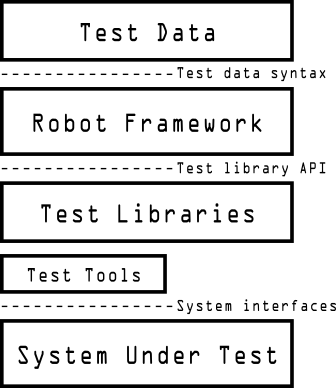
\includegraphics[width=0.4\textwidth]{assets/robot-arkkitehtuuri.png}
      \caption{Robot Framework alustan arkkitehtuuri \parencite{robot_framework_architecture}}
      \label{fig:robot-architecture}
    \end{figure}

    Robot Framework:illä rakennettuja testitapauksia voidaan ajaa komentoriviltä sen tarjoamalla robot-komennolla.
    Testitapauksien ajaminen tulostaa komentoriville yksinkertaisen raportin testitapauksen onnistumisesta ja lisäksi tallettaa varsin yksityiskohtaisen ja selkeän testitaportin ajetuille testitapauksille.
    Testiraportit ovat erittäin hyvin tehtyjä ja HTML-pohjaisia, joka tarkoittaa, että ne voidaan helposti integroida osaksi jatkuvan integraation koontiputkia.

    Yhtenä heikkoutena Robot Framework:issa on tuen puuttuminen ohjelmistokieliä hyödyntävillä testialustoilla löytyville kontrollirakenteille, joita esiintyy esimerkiksi yksikkötestaukseen tarkoitetuissa testialustoilla.
    Robot Framework on selkeästi vain hyväksymistestauksen testitapauksien rakentamista varten tarkoitettu testialusta ja siinä se on erinomainen vaihtoehto testitapauksien rakentamiseen.

  \subsection{Selenium} \label{ch:08_selenium}

    Selenium on suosittu avoimen lähdekoodin työkalu ja kirjastokokoelma verkkoselainten automatisoimiseen.
    Ensisijaisesti se on tarkoitettu web-sovelluksien automatisoimiseen testaustarpeita varten.
    Erityisen hyvin Selenium soveltuu hyväksymistestauksen testiautomaation rakentamiseen, sillä sen avulla automatisoidaan web-sovelluksien käyttöliittymissä tehtäviä toimenpiteitä.
    Selenium on ThoughtWorks yhtiön kehittämä verkkoselainten automatisoimiseen tarkoitettu työkalujen ja kirjastojen kokoelma ja se on saatavilla Windows, Linux ja MacOS käyttöjärjestelmille \parencite{selenium_info_1}.
    Sama yhtiö on toteuttanut myös tässä diplomityössä myöhemmin esitettävän GoCD-ohjelmiston, jota voidaan käyttää jatkuvan integroimisen ja julkaiseminen rakentamiseen.

    Selenium tuoteperheeseen kuuluvat Selenium WebDriver, Selenium IDE ja Selenium Grid komponentit \parencite{selenium_info_2}.
    Selenium WebDriver on varsinainen web-sovelluksien automatisoimiseen käytettävä ohjelmisto, jota myös tässä diplomityössä Selenium tuotteista käytetään.
    Selenium IDE on kehitysympäristö ohjelmistokehittäjille ja testaajille, jota voidaan halutessaan käyttää testitapauksien rakentamiseen.
    Selenium Grid on järjestelmä, jonka avulla voidaan Selenium pohjaisten testitapauksien suorittaminen skaalautuvasti hajauttaa useille eri etäkoneille.
    Tässä diplomityössä ei ole käytetty Selenium Grid -järjestelmää vaan testitapauksien suorittamiseen tarvittavat ohjelmistot on säiliöity Docker-työkalua käyttäen, joka mahdollistaa tarvittaessa skaalautuvuuden.

    Selenium on todella tärkeä osa web-sovelluksien testiautomaation rakentamista, sillä se pohjimmiltaan mahdollistaa web-sovelluksien käyttöliittymien käsittelemisen automatisoidusti.
    Selenium-työkalua voidaan käyttää erityisesti hyväksymistestauksen testitapauksien automatisoimiseen suoraan Selenium IDE:n avulla nauhoittaen testitapauksia tai kirjoittaen ne Selenium-skriptauskielellä.
    Selenium on joustava työkalu ja se tarjoaa Selenium Client API -rajapinnan, jonka avulla sitä voidaan käyttää muistakin ohjelmointikielistä, kuten C\#, JavaScript tai Python.

    Tässä diplomityössä Selenium työkalua käytetään Robot Framework:in yhteyteen integroituna ulkoisena kirjastona.
    Robot Framework:ille on saatavilla SeleniumLibrary niminen kirjasto, josta löytyy Robot Framework:in syntaksin mukaisesti määritellyt avainsanat verkkoselainten ohjaamiseen Selenium-pohjaisesti.

  \subsection{Xvfb} \label{ch:08_xvfb}

    Xvfb, eli X Virtual Framebuffer, on X-näyt\-tö\-pal\-ve\-li\-men  protokollan toteuttava virtuaalinen X-näyt\-tö\-pal\-ve\-lin.
   X-näyt\-tö\-pal\-ve\-li\-men tehtävä on mahdollistaa graafisten ohjelmien toiminta käyttöjärjestelmän ytimen päällä, jossa X-palvelin ja X-asiakasohjelmat kommunikoivat keskenään sekä X-palvelin hoitaa ytimen kautta näytön ja syöttölaitteiden käsittelyn.
    Xvfb ei tulosta mitään näytölle, vaan kaikki näytölle normaalisti tulostuva graafisia käyttöliittymiä sisältävä sisältö on ajonaikaisessa tietokoneen muistissa.
    Xvfb toimii aivan kuten tavallinenkin X-näyt\-tö\-pal\-ve\-lin, eli vastaa X-ohjelmien pyyntöihin ja hoitaa niihin liittyvän tapahtumien ja virheiden käsittelyn.

    Xvfb soveltuu web-sovelluksien hyväksymistestauksen automatisointiin mahdollistaen päätteettömän testaamisen testitapauksille.
    Päätteetöntä testausta voidaan toteuttaa myös verkkoselaimiin rakennettujen ominaisuuksien avulla, mutta Xvfb:n suurena etuna niihin on se, että sitä voidaan käyttää mihin tahansa graafiseen ohjelmaan.
    Päätteettömän testauksen mahdollistaminen on erittäin tärkeää, sillä se mahdollistaa myös käyttöliittymätestauksen suorittamisen jatkuvan integroinnin palvelimilla, jossa ei graafista ympäristöä ajon aikana muuten olisi.

    Yhtenä Xvfb:n heikkoutena on, että se on saatavilla vain UNIX-pohjaisiinX-näyt\-tö\-pal\-ve\-li\-men sisältäviin käyttöjärjestelmiin, kuten Linux ja MacOS.
    Näin ollen esimerkiksi Windows-alustalla toimivaa Internet Explorer verkkoselainta ei voida natiivisti testata.

    Robot Framework:ille on saatavilla XvfbRobot niminen kirjasto, jota tämän diplomityön toteutuksessa käytettiin.
    XvfbRobot on kirjasto, josta löytyy Robot Framework:in syntaksin mukaisesti määritellyt avainsanat Xvfb-palvelimen kanssa kommunikoimiseen.

  \subsection{Docker} \label{ch:08_docker}

    Docker on säiliöintityökalu, jonka avulla on mahdollista määrittää, rakentaa ja ajaa säiliöiden muotoon konfiguroituja sovelluksia.
    Docker muistuttaa virtuaalikoneita, mutta se on kevyempi ja resurssien käytössä optimaalisempi, sillä se jakaa käyttöjärjestelmän ytimen eri säiliöiden kesken ja virtualisoi vain sovellusympäristön jonka säiliön määrittävä konfiguraatio sisältää.
    Säiliöiden sisään voidaan paketoida kaikki kokonaisen sovelluksen tarvitsemat ohjelmistot, kirjastot, ympäristöt, riippuvuudet ja itse sovelluksen ohjelmakoodi.
    Rakentamalla säiliön ja käynnistämällä sen, voidaan sitä käyttää konfiguraatioltaan samanlaisena eri ympäristöissä joissa Docker-ohjelmisto on saatavilla.

    \begin{figure}[H]
      \centering
      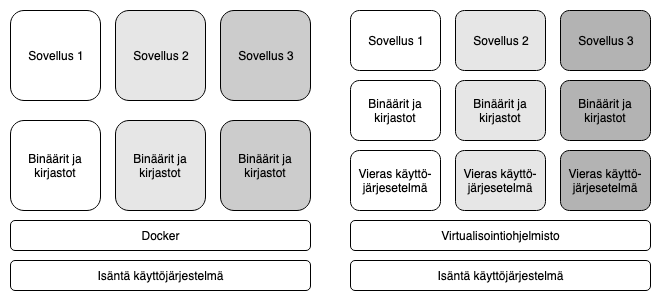
\includegraphics[width=0.8\textwidth]{assets/docker-vs-virtual-machine.png}
      \caption{Dockerin ja virtuaalikoneen vertailu}
      \label{fig:docker-vs-virtual-machine}
    \end{figure}

    Dockerfile:n avulla voidaan luoda räätälöity säiliö, josta voidaan rakentaa yksi tai useampia instansseja.
    Räätälöidyn säiliön etuna on etenkin se, että sen avulla saadaan aikaan sovellus joka on periaatteessa alustariippumaton.
    Sovelluskehittäjät voivat käyttää samaa Docker-konfiguraatiota rakentaakseen identtisiä säiliöitä sovelluskehityksen ajaksi, tarviten vain Docker-ohjelmiston.
    Tämän lisäksi Docker mahdollistaa saman Docker-konfiguraation käyttämisen sovelluksen pystyttämiseen ja julkaisemiseen nopeasti, helposti sekä jopa kustannustehokkaasti eri paikkoihin.
    Docker-compose on tapa rakentaa Docker-verkko, joka koostuu palveluista jotka ovat joko valmiiksi tehtyjä Docker-kuvia tai itse Dockerfile:n avulla tehtyjä Docker-kuvia.
    Docker-verkkoon voidaan myös lisätä yhteisiä tietosäilöjä, joita verkkoon kuuluvat palvelut voivat yhteisesti hyödyntää.
    Yksittäisen säiliön konfiguraation sisältämä Dockerfile ja kokonaisen Docker-verkon konfiguraation sisältämä docker-compose -tiedosto kirjoitetaan YAML-kielellä.

    Tässä diplomityössä Docker:ia käytettiin hyväksymistestauksen testitapauksien automatisoimiseen tarvittavien työkalujen säiliöinnissä.
    Olemassa olevaan Docker-verkkoon lisättiin hyväksymistestauksen testitapauksia varten tarkoitettu säiliö, joka hyödyntää Robot Framework:iä, Selenium:ia, Xvfb:ää ja sisältää muun muassa testauksessa tarvittavat verkkoselaimet.
    Docker:ia käyttämällä siis pystyttiin luomaan monistettava ja uniikki hyväksymistestauksen automatisointiympäristö, jota voidaan käyttää jatkuvan integraation yhteydessä testitapauksien suorittamiseen.

  \subsection{GoCD} \label{ch:08_gocd}

    GoCD on avoimen lähdekoodin jatkuvan integroinnin ja jatkuvan julkaisemisen mahdollistava palvelinohjelmisto.
    Ohjelmisto mahdollistaa koko koonti-testaus-julkaisu putkiryhmän tai vain sen osien automatisoimisen.
    GoCD-palvelinta mainostetaan soveltuvan hyvin erityisesti jatkuvan julkaisemisen rakentamiseen.
    GoCD on saman ThoughtWorks yhtiön kehittämä ohjelmisto, kuten aiemmin esitetty Selenium työkalukin \parencite{gocd_info}.

    Koonti-testaus-julkaisu putkiryhmän voi rakentaa GoCD-palvelimen graafisen käyttöliittymän kautta tai koodina käyttäen YAML tai JSON-syntaksia.
    Teknisesti GoCD-ohjelmisto koostuu itse palvelimesta ja agenteista, jotka voivat suorittaa palvelimen pyytämänä ennalta määritettyjä koonti-testaus-julkaisu putkiryhmän tehtäviä.
    Agentit ovat tarkoituksenmukaista sijoittaa eri järjestelmään kuin missä itse palvelin sijaitsee ja agenteille voi määrittää resurssiominaisuuksia, jotka kertovat palvelimelle mitä tehtäviä agenteilla voi teettää.
    GoCD-ohjelmiston terminologia on hieman tavallisesta poikkeavaa ja erilainen esimerkiksi todella suositun Jenkins-ohjelmiston vastaavista.
    GoCD-terminologiassa ylin käsite on putkiryhmä, jonka avulla yhteen kuuluvat putket voidaan järjestää samaan kokonaisuuteen.
    GoCD-terminologiassa yksittäinen putki vastaa esimerkiksi koontivaihetta tai testausvaihetta.
    Yksittäisen putken alaisuudessa on vaiheita, jotka antavat GoCD-palvelimen käyttöliittymässä tiedon vaiheen onnistumisesta.
    Vaiheet itsessään sisältävät vielä tehtäviä, jotka ovat yksittäisiä komentoja tai sellaisia suoritettavia tehtäviä, jotka agentit pystyvät käsittelemään.
    GoCD-ohjelmiston terminologiaan kuuluvat vielä vahvasti artefaktit, jotka ovat sellaisia tiedostoja mitä tehtävien suorittamisen yhteydessä syntyy ja jotka on merkitty säästettäväksi.
    Esimerkkejä artefakteista ovat ohjelman koontiversiot tai testiraportit.

    Jatkuvan integraation yhteydessä tapahtuvan testiautomaation puolesta ei välttämättä ole suurta merkitystä mikä jatkuvan integraation mahdollistava palvelinohjelmisto on käytössä.
    Tämä havainto tuli esiin, kun tätä diplomityötä varten testiautomaatioon tarvittavat ohjelmistot säiliöitiin aiemmin esitetyllä Docker-työkalulla, jota voidaan yhden testausvaiheen tehtävän aikana kutsua komentorivipohjaisesti.

\section{Testitapauksien rakentaminen} \label{ch:08_testitapauksien_rakentaminen}

  Testitapaus on testiautomaation näkökulmasta määritelty toimenpiteiden, ehtojen ja muuttujien joukko, joka suorittamalla voidaan verifioida jokin osa, ominaisuus tai toiminnallisuus ohjelmistosta.
  Testitapauksien rakentaminen on järkevää järjestää testikokoelmiksi, jotka tarkoittavan samaan kontekstiin kuuluvista testitapauksista muodostettua joukkoa.
  Tässä diplomityössä keskityttyyn hyväksymistestaukseen liittyen testitapaukset kirjoitetaan usein käyttötapauksien muodossa.
  Hyväksymistestauksen tapauksessa testitapauksien määrittäminen testiautomaatiota varten voidaan toteuttaa Robot Framework:illä ja apuna käyttää muita aiemmin mainittuja työkaluja.
  Lisäksi hyväksymistestauksen priorisoimiseen painotetun verkon avulla on välttämätöntä suunnitella ja rakentaa testitapaukset näkymä ja siirtymäperusteisesti, koska menetelmä hyödyntää matemaattisia näkymä ja siirtymäperusteisesti laadittuja painotettuja verkkoja.
  Tämän diplomityön liitteenä \ref{ch:12_liite_robot_testitapaus} on yksinkertaistettu esimerkki toteutettua hyväksymistestausjärjestelmää varten rakennetusta ja Robot Framework:iä käyttävästä testitapauksesta.

  Testitapauksen perusformaatti koostuu lähtötilanteesta, laukaisijasta ja verifikaatiosta.
  Lähtötilanteessa oletetaan jotakin ja seuraavassa vaiheessa seurataan, kun jokin ehto tapahtuu, jonka jälkeen voidaan tarkistaa seuraus ja verifioida onko se oletuksen mukainen.
  Testitapauksien yleisiä tavoitteita ovat: yksinkertaisuus, läpinäkyvyys, käyttäjätietoisuus, epätoistuvuus, olettamattomuus, kattavuus, tunnistettavuus, jälkensä puhdistava, toistettava, syvyyttömyys ja atomisuus \parencite{test_case_goals}.

  Robot Framework:in perustaja on kirjoittanut laajan ohjeistuksen siitä, miten Robot Framework:iä käyttäen luodaan hyviä testitapauksia \parencite{robot_framework_good_test_cases}.
  Klärckin ohjeistuksen pohjalta on huomioitavaa erityisesti testikokoelmien, testitapauksien ja avainsanojen nimeäminen jonka kuuluisi olla selkeää, kuvaavaa ja ytimekästä.
  Dokumentaation määrää testitapauksissa tulisi rajoittaa, sillä hyvin kirjoitetut testitapaukset ovat Robot Framework:iä käyttäen selkeitä jo sellaisenaan.
  Dokumentaatiota kuuluisi lisätä lähinnä vain testikokoelmiin yleisellä tasolla.
  Testikokoelmat kuuluisi sisältää vain toisiinsa liittyviä testejä ja testitapauksien sekä avainsanojen tulisi olla sellaisinaan selkeästi ymmärrettäviä.
  Muuttujien käytöllä suositellaan kapseloimaan pitkiä ja kompleksisia arvoja, mutta arvojen syöttäminen ja palauttaminen muuttujia hyödyntäen tulisi pitää pois testitapauksien tasolta.

\section{Priorisointiongelma} \label{ch:08_priorisointiongelma}

  Testitapauksien priorisointi on kustannussyistä tai resurssien optimoinnin kannalta erittäin tärkeää.
  Ohjelmistotestauksessa on myös hyvä tiedostaa, että ohjelmistotuotetta ei usein voida testata täydellisesti, joka nostaa esiin tarpeen tärkeimpien testitapauksien priorisoimisesta.
  Priorisoinnin toteuttamisen tärkeys korostuu erityisesti silloin kun kohdejärjestelmä on kompleksinen ja toiminnallisia ominaisuuksia on paljon.
  Priorisointi vaatii kuitenkin priorisointimenetelmästä riippumatta ylimääräistä työtä ohjelmistokehittäjiltä ja testaajilta.

  Priorisointiongelmaa voidaan ajatella sen laiminlyömisestä seuraavien haittojen näkökulmasta.
  Ilman testitapauksien priorisointia voi esiintyä muun muassa seuraavia haittoja.
  Prioriteettien puuttumisen seurauksena tärkeät ongelmat voidaan havaita vasta liian myöhään.
  Testitapauksia ei voida järjestää prioriteettien mukaan suoritettaviksi.
  Prioriteettijärjestyksen puuttumisesta johtuen epäoleellisten testitapauksien mukaan katkeava testaus voi piilottaa oleellisia testitapauksia.
  Tämän lisäksi myös prioriteettien puolesta epäoleellisetkin testitapaukset toteutetaan.
  Epäoleellisten testitapauksien toteuttaminen puolestaan kuluttaa resursseja ja lisää kustannuksia.
  Ajan myötä ohjelmistot ja niiden testaukseen toteutetut testitapaukset muuttuvat ja vanhenevat.
  Prioriteettien puuttuminen poistaa mahdollisuuden varautua oleellisten testitapauksien huolellisempaan ja aikaa kestävään suunnitteluun.
  Lisäksi testikattavuutta ei voida optimoida vähentämällä täysin epäoleellisia testitapauksia, jos niitä varten ei ole tehty priorisointia ennen toteutusta.

  Priorisointiongelman ratkaisemiseen on olemassa useita erilaisia lähestymistapoja ja menetelmiä, kuten esimerkiksi heuristinen priorisointi tai MoSCoW-menetelmä.
  Tässä diplomityössä esitetään ja käytetään priorisointiin kuitenkin vain matemaattista painotettuihin verkkoihin perustuvaa lähestymistapaa, joka on uudenlainen tämän diplomityön tuotteena kehittynyt matemaattinen menetelmä priorisointiongelman ratkaisemiseen.
